\documentclass[11pt]{beamer}
\usepackage[utf8]{inputenc}
\usepackage[T1]{fontenc}
%\usepackage{natbib}
\usetheme{Pittsburgh}
\usepackage{verbatim} 
\usepackage[english]{babel}
\usepackage{epstopdf}
\usepackage{multicol}
\usepackage{econometrics}
%\titlegraphic{%\vspace*{1cm}
%	\includegraphics[width=2.5cm]{logo_udelar}
	%\hspace*{1cm}~%
%		\includegraphics[width=3.5cm]{logo_FCEA.png}
%}

\setbeamercolor{block body alerted}{bg=alerted text.fg!10}
\setbeamercolor{block title alerted}{bg=alerted text.fg!20}
\setbeamercolor{block body}{bg=structure!10}
\setbeamercolor{block title}{bg=structure!20}
\setbeamercolor{block body example}{bg=green!10}
\setbeamercolor{block title example}{bg=green!20}


\setbeamertemplate{navigation symbols}{}
\setbeamertemplate{footline}[frame number]
\AtBeginSection{ 
	\begin{frame}
		\frametitle{Index}
			\tableofcontents[currentsection]
	\end{frame}
}
\begin{document}
	\title{Modelos dinámicos y computacionales en Economía}
	\subtitle{Modelos Basados en Agentes: Distribución}
	%\logo{}
	\institute{Licenciatura en Economía, FCEA, UDELAR}
	\date{21 de noviembre de 2024}

	%\subject{}
	%\setbeamercovered{transparent}
	%\setbeamertemplate{navigation symbols}{}
	\frame[plain]{
	\begin{figure}
	\centering
	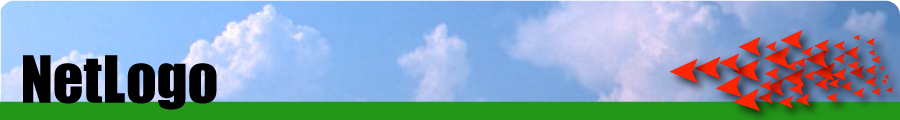
\includegraphics[width=0.7\linewidth]{figuras/netlogo-title-wide-60}
	%		\caption{}
	\label{fig:netlogo-title-wide-60}
\end{figure}	
		\vspace{-1cm}
\maketitle
}
%\setbeamertemplate{background}{\includegraphics[width=2 cm]{logo_FCEA.png}}


\begin{frame}
\frametitle{La complejidad de las ciencias sociales}
\begin{itemize}
	\item Los procesos sociales son complejos.
	\item No podemos realizar experimentos.
    \begin{itemize}
        \item Testeo de hipótesis.
	\item Efecto de políticas
    \end{itemize}
	\item Dificultad para relacionar comportamientos individuales con regularidades macroeconómicas
    \begin{itemize}
        \item Homogeneizar agentes (modelos de crecimiento macro)
	\item Fenomenología de patrones macro (modelos SIR, Lokta-Volterra)
    \end{itemize}
\end{itemize}
\end{frame}


\begin{frame}
\frametitle{Sociedad artificial}
\framesubtitle{\href{https://wtf.tw/ref/epstein_axtell.pdf}{Growing Artificial Societies: Social Science from the bottom-up}\footnote{\scriptsize{Epstein, J. M., \& Axtell, R. (1996). \textit{Growing artificial societies: social science from the bottom up.} Brookings Institution Press.}}}
\begin{itemize}
	\item Proponen "germinar" computacionalmente una sociedad artificial que permite estudiar diversas esferas de la actividad humana, combinando nociones de varias disciplinas (economía, demografía, etc).
	\item ¿Qué es una sociedad artificial? Un ABM de los procesos sociales.
	\item Laboratorio donde podemos experimentar y dilucidar los micro mecanismos que son \textit{suficientes} para generar las estructuras sociales y el comportamiento colectivo observable.
\end{itemize}
\end{frame}

\begin{frame}
\frametitle{Sugarspace vs. Modelos tradicionales}
\begin{itemize}
	\item Poblaciones de agentes heterogéneos: en los SIR, los Recuperados son todos iguales entre sí.
	\item Dimensión espacial.
	\item Interacción e información local: racionalidad limitada de Herbert Simon.
	\item Lo único constante es el cambio: no se asume a priori la existencia de un equilibrio. La dinamica misma del sistema es lo interesante.
	\item Más allá del individualismo metodológico: se parte de los individuos y su comportamiento, pero el sistema no queda sobredeterminado por ello.
	\item Estructuras colectivas emergentes: precios, tribus, migraciones, distribuciones estables de riqueza, etc.
\end{itemize}
\end{frame}


\begin{frame}
\frametitle{SugarScape}
\framesubtitle{Breve introducción}
\begin{itemize}
	\item Uno de los primeros Modelos Basados en Agentes (ABM) a gran escala.
	\item Consiste en una serie de modelos basados en una población con visión limitada y con recursos disponibles que se encuentran distribuidos en un espacio de dos dimensiones.
	\item El azúcar es una metáfora de los recursos en este mundo simulado, a través del cual podemos analizar los efectos de distintas dinámicas sociales.
\item Este trabajo fue la inspiración para una serie de ``modelos generativos'', lo que hizo crecer el campo de los ABM en economía y en las Ciencias sociales en general. 
%\item Es una metodología especialmente útil para la economía del comportamiento: se utilizan modelos con racionalidad limitada, cuyos agentes no tienen información completa y utilizan atajos o heurísticas para tomar decisiones.
	%\item Los agentes también pueden contaminar, morir, reproducirse, heredar recursos, transferir información, comerciar azúcar o transmitir enfermedades.
\end{itemize}
\end{frame}
	


\begin{frame}
\frametitle{Sugarspace}
\framesubtitle{Elementos}

\textbf{Entorno}:
medio con el cuál los agentes interactúan y donde desarrollan su actividad.
\begin{itemize}
	\item El sistema se desenvuelve en un espacio $\mathbb{R}^2$.
	\item Cada parche tiene un nivel de azúcar y una capacidad máxima.
	\item El mundo es un toro de $50 \times 50$.
\end{itemize}

\textbf{Agentes}:
autómatas celulares con reglas/heurísticas simples de comportamiento y atributos.
\begin{itemize}
	\item Acumulan y consumen azúcar para vivir.
	\item Metabolismo y visión asignados aleatoriamente (atributos).
	\item La visión es hasta donde pueden ver a su alrededor (vertical y horizontal).
	\item El metabolismo es cuánta azúcar necesita para subsistir en cada iteración.
	\item Al comienzo se les asigna una dotación inicial de azúcar.
\end{itemize}
\end{frame}

\begin{frame}
\frametitle{Sugarspace}
\framesubtitle{Reglas}
\begin{itemize}
	\item Los agentes consumen y acumulan $\Rightarrow$ regla para regenerar el azúcar.
	\begin{itemize}
		\item $G_{\infty}$ = en cada turno se regenera de inmediato.
		\item $G_{\alpha}$ = en cada turno se regeneran $\alpha$ unidades hasta alcanzar la capacidad máxima.
	\end{itemize}
	\item Movimiento: los agentes miran a su alrededor y se mueven al espacio desocupado y más cercano con mayor azúcar. En cada turno se mueven una sola vez.
	\item Los agentes mueren si su nivel de azúcar es 0 o menos.
\end{itemize}
\vspace{4mm}

Abrir el modelo en NetLogo: \textbf{Archivo / Biblioteca de Modelos / Sample Models / Social Science / Economics / Sugarscape / \\ "Sugarscape 1 Immediate Growback"}
\end{frame}



\begin{frame}
\frametitle{SugarScape}
\framesubtitle{Código}
\begin{itemize}
	\item En este caso, notar que existen variables globales, variables que afectan a los agentes y variables que afectan a los patches.
	\item Procedimientos:
	\begin{itemize}
		\item Se encuentran presentes SETUP y GO, junto con otros que son más específicos.
		\item Específicos de los patches (setup-patches, patch-growback, patch-recolor)
		\item Específicos de los agentes (turtle-setup, turtle-move, turtle-eat)
	\end{itemize}
\end{itemize}
\end{frame}

\begin{frame}
\frametitle{SugarScape}
\framesubtitle{Interfaz}
\begin{itemize}
	\item Podemos visualizar la población inicial y las cantidades mínima y máxima de riqueza (azúcar) inicial.
	\item También se observan gráficos de la vision y el metabolismo medio.
	
\end{itemize}
\end{frame}



\begin{frame}
	\label{g-inf}
\frametitle{Resultados}
\framesubtitle{$G_{\infty}$}
\begin{itemize}
	\item Luego de pocos turnos, los agentes se quedan quietos por su visión limitada. No ven una mejor posición y como el recurso se regenera por completo en cada turno, no es eficiente moverse.
	\item Algunos mueren. Sin haber fijado una \hyperlink{carry-cap}{capacidad de carga} del sistema, esta emerge de la propia dinámica del modelo.
	\item Los agentes con menor metabolismo y mayor visión son los que tienen más chances de sobrevivir. Se verifica cierta selección natural.
\end{itemize}

\end{frame}


\begin{frame}
\frametitle{Distribución de la riqueza}

Para poder estudiarla, es necesario modificar levemente el modelo anterior.
\begin{itemize}
	\item Si los agentes viven eternamente, no se alcanza una distribución estable, simplemente acumulan indefinidamente $\Rightarrow$ a cada agente le asignamos aleatoriamente una edad máxima del intervalo $[a,b]$.
	\item Debemos añadir una regla de reproducción de los agentes $\Rightarrow$ cada agente que muere es reemplazado por otro de edad 0 con atributos, dotación inicial de azúcar, posición y edad máxima aleatorias.
	
\end{itemize}

Como conocemos la riqueza de cada uno de los agentes, podemos graficar la curva de Lorenz y la evolución del índice de Gini.
\end{frame}

\begin{frame}
\frametitle{Resultados}
\framesubtitle{$G_1$ \& Edad máxima}
\begin{itemize}
	\item Los agentes zumban alrededor de una posición. Es eficiente porque se mueven de forma tal que permiten regenerar el parche donde estuvieron para después volver.
	\item Inicialmente la distribución de la riqueza es bastante simétrica pero rápidamente emerge una asimétrica.
	\item Con el índice de Gini y la curva de Lorenz vemos como empezamos con una sociedad casi perfectamente igualitaria pero en pocos turnos la curva de Lorenz se aleja de la línea 45°.
\end{itemize}

Es similar a lo que observamos en la \textit{realidad}. ¿Implica una ley natural inmutable? 
Podríamos agregar un impuesto progresivo al azúcar y/o una renta básica, y ver que patrones emergen.

\end{frame}




\begin{frame}
\frametitle{SugarScape}
\framesubtitle{Extensiones y modificaciones}


\begin{itemize}
	\item ¿Cantidad mínima y máxima de azúcar inicial?
	\item ¿Metabolismo?
	\item ¿Visión?
	\item ¿Cantidad de azúcar que obtienen del patch? ($G_{\alpha}$)
\end{itemize}

\vspace{3mm}
A través del libro, se van incorporando nuevas reglas de comportamiento que complejizan al modelo.

\begin{itemize}
	\item Sexo, cultura y conflicto: proto-historia, reproducción sexual, dinámica poblacional, formación de tribus, conflicto.
	\item Comercio: se agrega otro recurso, la "especia" para ver los procesos de formación de precios. Se permite el comercio bilateral de recursos.
	\item Enfermedades: contagio y difusión.
\end{itemize}
\end{frame}

\begin{frame}
	FIN :)
\end{frame}

\begin{frame}
	\label{carry-cap}
	\frametitle{\hyperlink{g-inf}{Capacidad de carga}}
	\framesubtitle{En función de la visión media y distintos valores de metabolismo}

	Bajo las reglas $G_{1},M$ y distribuciones aleatorias de los agentes.
	\vspace{3mm}
	
	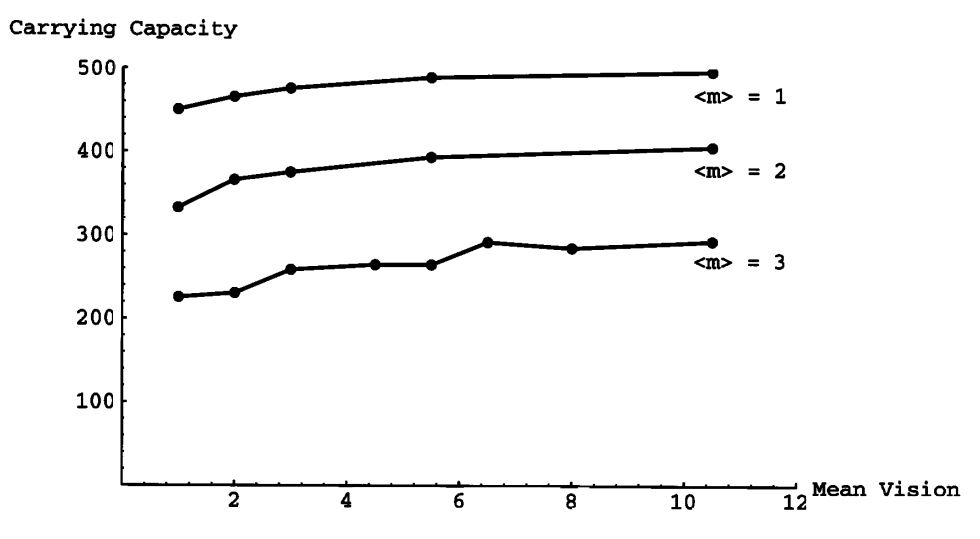
\includegraphics[width=1\linewidth]{figuras/carry_capacity.JPG}

	

\end{frame}

\end{document}
